\documentclass{article}
\usepackage[spanish]{babel}
	\deactivatetilden
\spanishdecimal{.}
\addto\captionsspanish{\def\tablename{Tabla}}
\addto\captionsspanish{\def\listtablename{\'Indice de tablas}}
\usepackage[numbers,sort&compress]{natbib}
\usepackage[T1]{fontenc}
\usepackage[utf8]{inputenc}
\usepackage{graphicx}
\usepackage{url}
\usepackage{graphicx}
\graphicspath{{Figuras/}}
\usepackage[numbers,sort&compress]{natbib}
\usepackage[clearempty,pagestyles]{titlesec}
\usepackage{anysize}
\usepackage{xcolor, colortbl}
\usepackage{array, multirow, multicol}
\usepackage{enumerate} 

\def\baselinestretch{1.5}
\papersize{27.9cm}{21.5cm} 
\marginsize{2cm}{2cm}{1cm}{1cm}

\title {Diagramas de Voronoi}
\author{Julio Garc\'ia}
\pagestyle{empty}

\pagestyle{empty}

\begin{document}
	\renewcommand{\listtablename}{Índice de tablas}
	\renewcommand{\tablename}{Cuadro}
\maketitle
	
\section{Introducción}
En el presente trabajo se busca como objetivo principal el estudio los diagramas de Voronoi con aplicaciones principalmente en el área de materiales, haciendo uso de la Simulación. El diagrama de Voronoi sirve para dividir un campo en regiones, de forma que cada región sabrá que todos los puntos contenidos en ella están más cerca de la semilla de esa región que de cualquier otra semilla. Dentro de las aplicaciones más conocidas de este tipo de diagramas se encuentra el diagnóstico de tumores, evitar colisiones de barcos en la costa y estudio de propagación de fracturas en un material.\\
\\
En la tarea 4 se busca estudiar el efecto que se tiene la variación de numero de semillas y de la zona de distribución de una grieta en términos de la distancia euclidiana entre la grieta y el exterior de la pieza.

\section{Desarrollo}
En este trabajo se busca analizar el siguiente problema: Examina de manera sistemática el efecto del número de semillas y del tamaño de la zona en la distribución en las grietas que se forman en términos de la mayor distancia euclideana entre la grieta y el exterior de la pieza. 
El código de este trabajo usa como base los códigos encontrados en el documento de la Práctica 4: Diagramas de Voronoi hechos por la Dra. Shaeffer \cite{p4}, modificando el numero de semillas en el campo y el tamaño de la grieta. 

Se realizaron variaciones de semillas con:  20,30,40 semillas; y con: 10 y 20 réplicas.

\section{Experimentación y resultados}
En esta sección se describe el ambiente computacional y los resultados obtenidos con la simulación. El código de dicha simulación fue realizado en el lenguaje computacional Python, en una computadora personal con procesador 1 Intel Core i7, con memoria RAM de 16GB y hasta 8 núcleos de procesamiento. Dicho código fue incorporado en el repositorio \cite{p_4}. 
Como se mencionó anteriormente se realizaron variaciones de semillas con:  20,30,40 semillas; y con: 10 y 20 réplicas.\\
\\
En la realidad, uno de los principales problemas ocasionado por una grieta, es cuantificar el daño causado por dicha grieta. Normalmente, este daño es medido a través de la profundidad de dicha grieta comparado con los ejes. A continuación, se definen las siguientes métricas para tratar de simular dicho efecto:\\
\\
Las métricas utilizadas están dadas de la siguiente manera:\\
\\
\textbf{Métrica 1}: Distancia euclidiana entre la grieta y el exterior de la pieza. Dicha distancia se obtiene calculando el mínimo de todas las distancias de cada punto de grieta al exterior de la pieza. A cada punto se le calculan 4 distancias para obtener la distancia al marco superior, inferior, derecho e izquierdo acorde a la siguiente imagen, la distancia del punto al marco de la pieza es el máximo de estas 4 distancias:\\
\\
\begin{figure}[h]
	\centering
	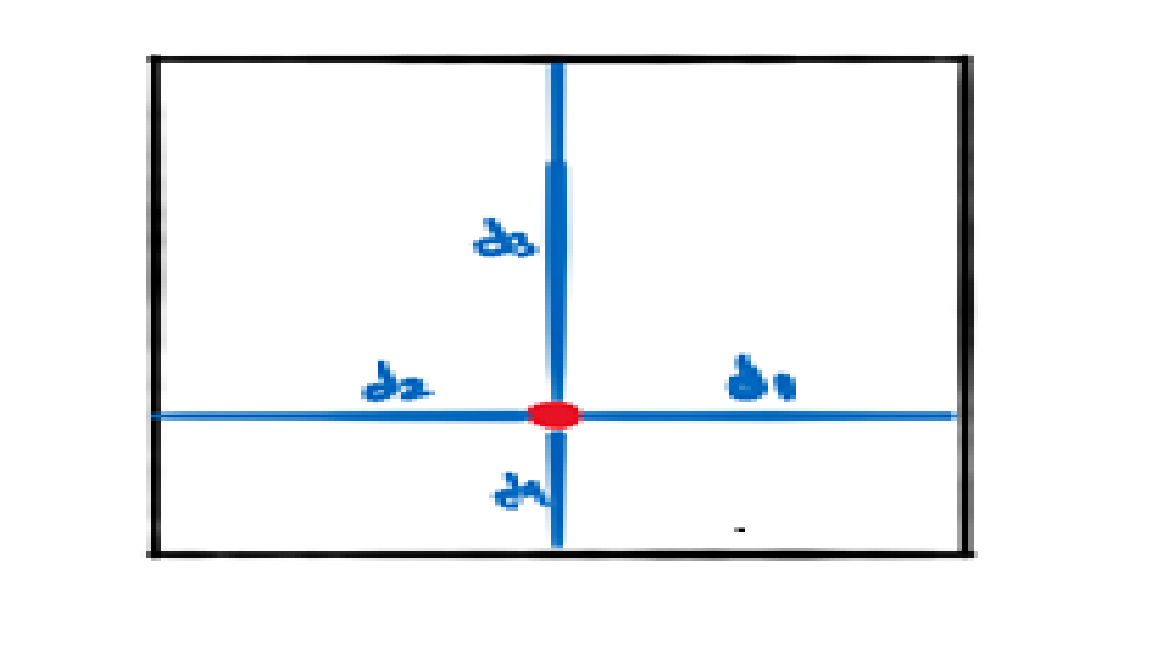
\includegraphics[width=0.7\linewidth]{imagen1}
	\caption{Métrica 1}
	\label{fig:imagen1}
\end{figure}
\\

\textbf{Métrica 2}: Distancia euclidiana entre el punto central del campo y la grieta. Se propone esta métrica como una segunda medición de qué tan profunda (cerca del centro del campo) fue la grieta simulada.  Pc representa el punto central del campo, Pg representa un punto de la grieta.\\
\\
\newpage
\begin{figure}[h]
	\centering
	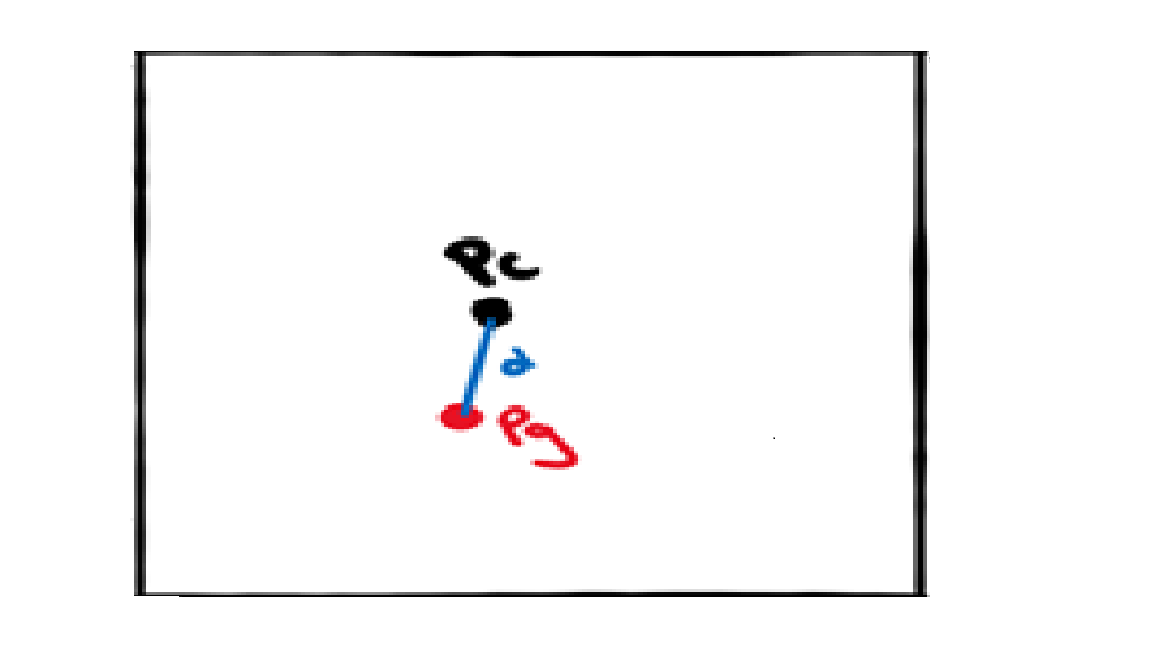
\includegraphics[width=0.7\linewidth]{imagen2}
	\caption{Métrica 2}
	\label{fig:imagen2}
\end{figure}



Se muestran los resultados en las siguientes tablas.\\

\begin{center}

\begin{table}[htbp]
	\centering
	\caption{Resultados  de las métricas 1 y 2 con 20 semillas  y 10 replicas}
	\begin{tabular}{|c|c|c|}
		\hline
		Experimento  & \multicolumn{1}{l|}{Métrica 1} & \multicolumn{1}{p{6.835em}|}{Métrica 2} \\
		\hline
		\multicolumn{1}{|r|}{1} & 71    & 23.632 \\
		\hline
		\multicolumn{1}{|r|}{2} & 66    & 43.846 \\
		\hline
		\multicolumn{1}{|r|}{3} & 63    & 82.901 \\
		\hline
		\multicolumn{1}{|r|}{4} & 76    & 81.991 \\
		\hline
		\multicolumn{1}{|r|}{5} & 69    & \cellcolor[rgb]{ .663,  .816,  .557}16.688 \\
		\hline
		\multicolumn{1}{|r|}{6} & 49    & 24.668 \\
		\hline
		\multicolumn{1}{|r|}{7} & 64    & 83.501 \\
		\hline
		\multicolumn{1}{|r|}{8} & 66    & 24.423 \\
		\hline
		\multicolumn{1}{|r|}{9} & 64    & 75.474 \\
		\hline
		\multicolumn{1}{|r|}{10} & \cellcolor[rgb]{ .663,  .816,  .557}44 & 42.101 \\
		\hline
		Promedio & 63.2  & 49.923 \\
		\hline
		Min   & 44    & 16.688 \\
		\hline
	\end{tabular}%
	\label{tab:cuadro1}%
\end{table}%




%%%%%%%%%%%%%%%%%%%%%%%%%%%%%%%%

\begin{table}[htbp]
	\centering
	\caption{Resultados  de las métricas 1 y 2 con 30 semillas  y 10 replicas}
	\begin{tabular}{|c|c|c|}
		\hline
		Experimento  & \multicolumn{1}{l|}{Métrica 1} & \multicolumn{1}{l|}{Métrica 2} \\
		\hline
		\multicolumn{1}{|r|}{1} & 51    & 40.577 \\
		\hline
		\multicolumn{1}{|r|}{2} & 58    & \cellcolor[rgb]{ .663,  .816,  .557}21.272 \\
			\hline
		\multicolumn{1}{|r|}{3} & 75    & 106.060 \\
			\hline
		\multicolumn{1}{|r|}{4} & 51    & 33.771 \\
		\hline
		\multicolumn{1}{|r|}{5} & \cellcolor[rgb]{ .663,  .816,  .557}47 & 66.47179 \\
			\hline
		\multicolumn{1}{|r|}{6} & 62    & 26.086 \\
			\hline
		\multicolumn{1}{|r|}{7} & 73    & 74.111 \\
			\hline
		\multicolumn{1}{|r|}{8} & 55    & 54.208 \\
			\hline
		\multicolumn{1}{|r|}{9} & 62    & 76.814 \\
			\hline
		\multicolumn{1}{|r|}{10} & 53    & 41.382 \\
			\hline
		Promedio & 58.7  & 54.075 \\
			\hline
		Min   & 47    & 21.272 \\
			\hline
	\end{tabular}%
	\label{tab:cuadro2}%
\end{table}%

%%%%%%%%%%%%%%%%%%%%%%
\begin{table}[htbp]
	\centering
	\caption{Resultados  de las métricas 1 y 2 con 40 semillas  y 10 replicas}
	\begin{tabular}{|c|c|c|}
		\hline
		\multicolumn{1}{|l|}{Experimento } & \multicolumn{1}{l|}{Métrica 1} & \multicolumn{1}{p{5.39em}|}{Métrica 2} \\
		\hline
		1     & 71    & 70.8978 \\
		\hline
		2     & 56    & \cellcolor[rgb]{ .663,  .816,  .557}46.2222 \\
		\hline
		3     & 71    & 65.5171 \\
		\hline
		4     & 75    & 84.7614 \\
		\hline
		5     & \cellcolor[rgb]{ .663,  .816,  .557}54 & 48.8108 \\
		\hline
		6     & 74    & 87.2954 \\
		\hline
		7     & 65    & 59.6699 \\
		\hline
		8     & 73    & 80.9845 \\
		\hline
		9     & 72    & 75.5546 \\
		\hline
		10    & 72    & 58.5021 \\
		\hline
		\multicolumn{1}{|l|}{Promedio} & 68.3  & 67.82158 \\
		\hline
		Min & 54    & 46.2222 \\
		\hline
	\end{tabular}%
	\label{tab:addlabel}%
\end{table}%

\begin{table}[htbp]
	\centering
	\caption{Resultados  de las métricas 1 y 2 con 20 semillas  y 20 replicas}
	\begin{tabular}{|c|c|c|}
		\hline
		Experimento  & \multicolumn{1}{l|}{Métrica 1} & \multicolumn{1}{p{6.835em}|}{Métrica 2} \\
		\hline
		\multicolumn{1}{|r|}{1} & 74    & 86.7784 \\
		\hline
		\multicolumn{1}{|r|}{2} & 77    & \cellcolor[rgb]{ .663,  .816,  .557}0.7071 \\
		\hline
		\multicolumn{1}{|r|}{3} & 72    & 77.7978 \\
		\hline
		\multicolumn{1}{|r|}{4} & 65    & 55.5562 \\
		\hline
		\multicolumn{1}{|r|}{5} & 76    & 76.58 \\
		\hline
		\multicolumn{1}{|r|}{6} & 68    & 75.5016 \\
		\hline
		\multicolumn{1}{|r|}{7} & 73    & 98.4504 \\
		\hline
		\multicolumn{1}{|r|}{8} & 57    & 76.1347 \\
		\hline
		\multicolumn{1}{|r|}{9} & 74    & 27.5045 \\
		\hline
		\multicolumn{1}{|r|}{10} & 77    & 82.2344 \\
		\hline
		\multicolumn{1}{|r|}{11} & 57    & 31.5356 \\
		\hline
		\multicolumn{1}{|r|}{12} & 62    & 56.5022 \\
		\hline
		\multicolumn{1}{|r|}{13} & \cellcolor[rgb]{ .663,  .816,  .557}55 & 24.135 \\
		\hline
		\multicolumn{1}{|r|}{14} & 72    & 49.5025 \\
		\hline
		\multicolumn{1}{|r|}{15} & 75    & \cellcolor[rgb]{ .663,  .816,  .557}0.7071 \\
		\hline
		\multicolumn{1}{|r|}{16} & 77    & 83.2856 \\
		\hline
		\multicolumn{1}{|r|}{17} & 65    & 12.349 \\
		\hline
		\multicolumn{1}{|r|}{18} & 69    & 86.7784 \\
		\hline
		\multicolumn{1}{|r|}{19} & 70    & 30.6022 \\
		\hline
		\multicolumn{1}{|r|}{20} & 62    & \cellcolor[rgb]{ .663,  .816,  .557}0.7071 \\
		\hline
		Promedio & 68.85 & 51.66749 \\
		\hline
		Min   & 55    & 0.7071 \\
		\hline
	\end{tabular}%
	\label{tab:cuadro 4}%
\end{table}%

\begin{table}[htbp]
	\centering
	\caption{Resultados  de las métricas 1 y 2 con 30 semillas  y 20 replicas}
	\begin{tabular}{|c|c|c|}
		\hline
		Experimento  & \multicolumn{1}{l|}{Métrica 1} & \multicolumn{1}{l|}{Métrica 2} \\
		\hline
		\multicolumn{1}{|r|}{1} & 75    & 93.7043 \\
		\hline
		\multicolumn{1}{|r|}{2} & 69    & 54.8862 \\
		\hline
		\multicolumn{1}{|r|}{3} & 53    & 38.5032 \\
		\hline
		\multicolumn{1}{|r|}{4} & 70    & 11.5974 \\
		\hline
		\multicolumn{1}{|r|}{5} & 75    & \cellcolor[rgb]{ .663,  .816,  .557}7.5166 \\
		\hline
		\multicolumn{1}{|r|}{6} & 62    & 76.4885 \\
		\hline
		\multicolumn{1}{|r|}{7} & 74    & 70.5443 \\
		\hline
		\multicolumn{1}{|r|}{8} & 71    & 50.5222 \\
		\hline
		\multicolumn{1}{|r|}{9} & 61    & 51.2298 \\
		\hline
		\multicolumn{1}{|r|}{10} & 46    & 44.9054 \\
		\hline
		\multicolumn{1}{|r|}{11} & 69    & 19.5576 \\
		\hline
		\multicolumn{1}{|r|}{12} & 59    & 59.3 \\
		\hline
		\multicolumn{1}{|r|}{13} & 59    & 81.8077 \\
		\hline
		\multicolumn{1}{|r|}{14} & 74    & 74.783 \\
		\hline
		\multicolumn{1}{|r|}{15} & \cellcolor[rgb]{ .663,  .816,  .557}40 & 39.7555 \\
		\hline
		\multicolumn{1}{|r|}{16} & 54    & 10.6066 \\
		\hline
		\multicolumn{1}{|r|}{17} & 75    & 71.5856 \\
		\hline
		\multicolumn{1}{|r|}{18} & 48    & 42.0297 \\
		\hline
		\multicolumn{1}{|r|}{19} & 45    & 39.7555 \\
		\hline
		\multicolumn{1}{|r|}{20} & 62    & 55.5202 \\
		\hline
		Promedio & 62.05 & 49.729965 \\
		\hline
		Min   & 40    & 7.5166 \\
		\hline
	\end{tabular}%
	\label{tab:addlabel}%
\end{table}%


\begin{table}[htbp]
	\centering
	\caption{Resultados  de las métricas 1 y 2 con 40 semillas  y 20 replicas}
	\begin{tabular}{|c|c|c|}
		\hline
		Experimento  & \multicolumn{1}{l|}{Métrica 1} & \multicolumn{1}{p{5.39em}|}{Métrica 2} \\
		\hline
		\multicolumn{1}{|r|}{1} & 59    & 12.0208 \\
		\hline
		\multicolumn{1}{|r|}{2} & 75    & 80.0156 \\
		\hline
		\multicolumn{1}{|r|}{3} & 69    & 66.5169 \\
		\hline
		\multicolumn{1}{|r|}{4} & 57    & 77.1913 \\
		\hline
		\multicolumn{1}{|r|}{5} & 69    & 74.3807 \\
		\hline
		\multicolumn{1}{|r|}{6} & 73    & 67.7237 \\
		\hline
		\multicolumn{1}{|r|}{7} & 60    & 45.5686 \\
		\hline
		\multicolumn{1}{|r|}{8} & 61    & 59.0635 \\
		\hline
		\multicolumn{1}{|r|}{9} & 60    & 59.6699 \\
		\hline
		\multicolumn{1}{|r|}{10} & \cellcolor[rgb]{ .663,  .816,  .557}43 & 58.7068 \\
		\hline
		\multicolumn{1}{|r|}{11} & 77    & 15.508 \\
		\hline
		\multicolumn{1}{|r|}{12} & 73    & 20.506 \\
		\hline
		\multicolumn{1}{|r|}{13} & 69    & 46.5026 \\
		\hline
		\multicolumn{1}{|r|}{14} & 72    & 31.5039 \\
		\hline
		\multicolumn{1}{|r|}{15} & 71    & 89.9027 \\
		\hline
		\multicolumn{1}{|r|}{16} & 67    & 69.7316 \\
		\hline
		\multicolumn{1}{|r|}{17} & 57    & 69.7316 \\
		\hline
		\multicolumn{1}{|r|}{18} & 77    & \cellcolor[rgb]{ .663,  .816,  .557}0.7071 \\
		\hline
		\multicolumn{1}{|r|}{19} & 71    & 18.5067 \\
		\hline
		\multicolumn{1}{|r|}{20} & 67    & 71.4737 \\
		\hline
		Promedio & 66.35 & 51.746585 \\
		\hline
		Min   & 43    & 0.7071 \\
		\hline
	\end{tabular}%
	\label{tab:addlabel}%
\end{table}%

\end{center}
\newpage
\section{Conclusiones}
Tomando como referencia los resultados mostrados en la tabla con las variaciones en la cantidad de semillas y de tamaño mínimo de grieta podemos presentar las siguientes conclusiones:
\begin{enumerate}
\item Conforme va aumentando la cantidad de semillas en un campo va aumentando también dificultad con la que una grieta se propaga hacia el interior del campo, esto se refleja ya que alcanza puntos mas profundos del campo en el que se está trabajando cuando se tienen menos semillas, alcanzando en ocasiones incluso a agrietar muy cerca del centro de la figura. Esto se debe probablemente a que cuando hay una mayor cantidad de semillas se tiene por tanto una mayor cantidad de regiones y por tanto una mayor cantidad de puntos frontera por los cuales es más fácil que se expanda la grieta, sin embargo, como la grieta puede seguir muchos caminos diferentes, cada vez es menos probable que se vaya hacia el centro del campo.
\item Con respecto a la distancia entre la grieta y el exterior de la pieza se sigue un comportamiento similar al anterior cuando se realiza el experimento con 10 réplicas, sin embargo, el comportamiento no es consistente cuando hay 20 réplicas.

\end{enumerate}

\bibliography{Biblio}
\bibliographystyle{plainnat}

\end{document}